\subsection{Direct search methods}\label{direct-search}
Among direct search methods, we will describe the \textit{generalized pattern search} (hereafter GPS) method \cite{Audet2002} and the \textit{mesh adaptive direct search} (hereafter MADS) method \cite{Audet2006}.

To describe the GPS algorithm, it is necessary to define a mesh, which is used to describe the search sets within the GPS algorithm. Let $ \mathbf{G} \in \mathbb{R}^{n \times n} $ be invertible and $ \mathbf{Z} \in \mathbb{Z}^{n \times p} $, $n, p \in \mathbb{N}$. Assume that every vector from $ \mathbb{R}^{n} $ can be expressed as a linear combination of the columns of matrix $ \mathbf{Z} $ (treated as vectors), such that all the coefficients in this linear combination are non-negative. Furthermore, let $ \mathbf{D} = \mathbf{G} \mathbf{Z} $. The mesh $ \mathbf{M} $ generated by $ \mathbf{D} $ centered at point $ \vec{x} $ is defined as
\begin{equation}
	\mathbf{M} = \left\{ \vec{x} + \delta \, \mathbf{D} y \, | \, y \in \mathbb{N}^p \right\},
\end{equation}
where $ \delta $ is called the mesh size parameter \cite{BBO-textbook, Audet2002}. In each iteration of the GPS algorithm, the shape of the mesh generally changes, as it is always centered at the point representing the best estimate in that iteration, and the size of the mesh step also changes. Let $ \vec{x}_k $ and $ \delta_k $ represent the estimate of the solution and the mesh size in the $ k $-th iteration, respectively. We 
then define the mesh in the $ k $-th iteration, denoted as $ \mathbf{M} _k $, as
\begin{equation}
	\mathbf{M} _k = \left\{ \vec{x}_k + \delta_k \, \mathbf{S} y \, | \, y \in \mathbb{N}^p \right\}.
\end{equation}
Note that the columns of matrix $ \mathbf{D} $, as defined above, can be interpreted as the possible directions in which the GPS algorithm searches the optimization space \cite{BBO-textbook, Audet2002}. Examples of search directions and meshes generated by different matrices $\mathbf{G}$ and $\mathbf{Z}$ are presented in Figure~\ref{fig:gps}.


\begin{figure}[H]
	\centering
	\vspace{1cm}
	
\includegraphics[width=0.70\textwidth]{figures/gps.pdf}
	\caption{Examples of search directions and meshes in $\mathbb{R}^2$ with
		obtained by different choices of $\mathbf{G}$ and~$\mathbf{Z}$. The mesh points
		are at the intersections of the lines, the arrows represent possible search directions.}
	\label{fig:gps}
\end{figure}


After initializing the necessary starting parameters, each iteration of the GPS algorithm is divided into two main steps. The first step is called the search step. During the search step, a finite set $S_k$ of candidate mesh points, selected according to a strategy specified by the user, is evaluated by computing the objective function at each one of the points. If none of the evaluated points represents an improvement over the value $ f(\vec{x}_k) $, the poll step follows. In the poll step, the objective function is evaluated at all neighboring mesh points of $ \vec{x}_k $. If none of the evaluated points represents an improvement over the value $ f(\vec{x}_k) $, we set $ \vec{x}_{k+1} = \vec{x}_k $ and decrease the mesh size, i.e., $ \delta_{k+1} < \delta_k $. However, if a point that improves the estimate of the solution is found in either the search or the poll step, this point is set as $ \vec{x}_{k+1} $, and the mesh size is increased, i.e., $ \delta_{k+1} > \delta_k $ \cite{BBO-textbook, Audet2002}.

The changes described above define a new mesh $ \mathbf{M} _k $ in each iteration. The mesh changes throughout the GPS algorithm. The algorithm terminates when $ \delta_{k+1} < \varepsilon $ for some user-specified $ \varepsilon > 0 $. It can be shown that the mesh step converges to zero, and under appropriate assumptions, the solution estimates converge to a stationary point of the objective function. Details can be found in \cite{BBO-textbook}. It should be noted that the convergence of GPS has been proven for unconstrained problems \cite{BBO-textbook}. The full GPS algorithm is presented is presented in Algorithm~\ref{GPS-algo}.
\\[4pt]
\begin{algorithm}[H]
	\caption{Generalized Pattern Search (GPS) for unconstrained optimization}\label{GPS-algo}
	\begin{algorithmic}[1]
		\Require Function $f: \mathbb{R}^n \to \mathbb{R}$, initial point $x^0$, initial mesh size parameter $\delta^0$, positive spanning matrix $D$, mesh size adjustment parameter $\tau \in (0, 1)$, stopping tolerance $\epsilon_{\text{stop}}$, iteration counter $k \gets 0$
		\Ensure Approximate solution $x^*$
		
		\Procedure{GPS}{$x^0$}
		
		\While{$\delta^k > \epsilon_{\text{stop}}$}
		
		\Algphase{1. Search}
		\State Define a finite subset $S^k$ of the mesh $M^k$
		\If{$f(t) < f(x^k)$ for some $t \in S^k$}
		\State Set $x^{k+1} \gets t$ and $\delta^{k+1} \gets \tau^{-1} \delta^k$
		\State \textbf{continue}
		\Else
		\State Go to Poll step
		\EndIf
		
		\Algphase{2. Poll}
		\State Select a positive spanning set $D^k \subseteq D$
		\State Define $P^k = \{x^k + \delta^k d : d \in D^k\}$
		\If{$f(t) < f(x^k)$ for some $t \in P^k$}
		\State Set $x^{k+1} \gets t$ and $\delta^{k+1} \gets \tau^{-1} \delta^k$
		\Else
		\State $x^k$ is a mesh local optimizer
		\State Set $x^{k+1} \gets x^k$ and $\delta^{k+1} \gets \tau \delta^k$
		\EndIf
		
		\Algphase{3. Termination}
		\If{$\delta^{k+1} \leq \epsilon_{\text{stop}}$}
		\State \textbf{terminate}
		\Else
		\State Increment $k \gets k+1$ and continue
		\EndIf
		
		\EndWhile
		\EndProcedure
	\end{algorithmic}
\end{algorithm}

We will also briefly mention the MADS method, which represents an improvement over the GPS method. Unlike GPS, the MADS algorithm allows the exploration of the objective function's values in directions that form a dense subset in $ \mathbb{R}^{n} $ during the poll step \cite{BBO-textbook, derivative-free-review}. This generalization improves the convergence of the algorithm and allows for proving the convergence of MADS even for constrained problems, where the objective function is modified into an extreme barrier function \ref{eq:extreme barrier}. Details regarding the MADS algorithm and its operation can be found, for example, in \cite{BBO-textbook}.


\begin{figure}[H]
	\centering
	\includegraphics[width=1.01\textwidth]{figures/mads.pdf}
	\caption{Examples of meshes and frames $\mathbb{R}^2$ for different
		values of $\delta^k$ and $\Delta^k$}
	\label{fig:mads}
\end{figure}



\begin{algorithm}[H]
	\caption{Mesh Adaptive Direct Search (MADS)}\label{MADS}
	\begin{algorithmic}[1]
		\Require Function $f_{\Omega}: \mathbb{R}^n \to \mathbb{R} \cup \{\infty\}$, initial point $x^0 \in \Omega$, initial frame size parameter $\Delta^0$, positive spanning matrix $D$, mesh size adjustment parameter $\tau \in (0,1)$, stopping tolerance $\epsilon_{\text{stop}}$, iteration counter $k \gets 0$
		\Ensure Approximate solution $x^*$
		
		\Procedure{MADS}{$x^0$}
		
		\While{$\Delta^k > \epsilon_{\text{stop}}$}
		
		\Algphase{1. Parameter Update}
		\State Set the mesh size parameter $\delta^k = \min \{\Delta^k, (\Delta^k)^2\}$
		
		\Algphase{2. Search}
		\State Define a finite set $S^k \subset M^k$ such that:
		\If{$f_{\Omega}(t) < f_{\Omega}(x^k)$ for some $t \in S^k$}
		\State Set $x^{k+1} \gets t$ and $\Delta^{k+1} \gets \tau^{-1}\Delta^k$
		\State \textbf{continue}
		\Else
		\State Go to Poll step
		\EndIf
		
		\Algphase{3. Poll}
		\State Select a positive spanning set $D_{\Delta^k}$ and define:
		\State $P^k = \{x^k + \delta^k d : d \in D_{\Delta^k}\}$, a subset of the frame $F^k$ with extent $\Delta^k$
		\If{$f_{\Omega}(t) < f_{\Omega}(x^k)$ for some $t \in P^k$}
		\State Set $x^{k+1} \gets t$ and $\Delta^{k+1} \gets \tau^{-1}\Delta^k$
		\Else
		\State Set $x^{k+1} \gets x^k$ and $\Delta^{k+1} \gets \tau\Delta^k$
		\EndIf
		
		\Algphase{4. Termination}
		\If{$\Delta^{k+1} \leq \epsilon_{\text{stop}}$}
		\State \textbf{terminate}
		\Else
		\State Increment $k \gets k+1$ and continue
		\EndIf
		
		\EndWhile
		\EndProcedure
	\end{algorithmic}
\end{algorithm}